\section{基于 Unity 的森林 VR 场景构建与展示}

\subsection{实验目的与场景主题}

本章围绕 Unity 中的 VR 场景搭建过程展开，实验主题为森林环境。与前两章主要分析人脸识别模型和浏览器端推理流程不同，本章关注虚拟现实课程中的三维场景构建、资源导入、渲染兼容性处理和 VR 视角配置。实验目标是在 Unity 中创建一个可进入、可观察的森林 VR 场景，使用户能够通过 VR 视角进入自然环境，并在运行时观察地形、树木、草地和光照等空间元素。

森林主题适合作为 VR 场景实验对象。一方面，森林包含地形、植被、树叶、草丛、天空和光照等丰富视觉元素，可以较直观地展示三维环境的沉浸感；另一方面，植被资源通常依赖双面渲染、透明裁剪和阴影投射，对渲染管线兼容性有一定要求。因此，本实验不仅是简单地把模型拖入场景，还需要处理旧资源包导入 Unity 6 + Universal Render Pipeline 后出现的材质显示问题。

本章按照实际操作顺序记录实验过程：首先创建 Unity VR 模板项目，确认项目版本和渲染管线；然后从 Asset Store 导入 Fantasy Forest Environment Free Sample 资源包；接着分析并修复导入后场景大面积显示为粉色的问题；最后将 VR 模板场景中的 XR Origin 复制到森林样例场景中，完成 VR 视角的接入与运行展示。

\subsection{创建 Unity VR 模板项目}

\subsubsection{选择 VR 项目模板}

实验首先在 Unity Hub 中创建 VR 模板项目。与普通 3D 模板相比，VR 模板会预先配置 XR 相关依赖、输入系统、相机结构和交互组件，适合作为虚拟现实实验的起点。如果从普通 3D 项目开始，需要额外安装和配置 XR Plugin Management、XR Interaction Toolkit、Input System 等内容，配置过程更容易遗漏。使用 VR 模板可以把重点放在场景资源和运行展示上。

\begin{figure}[htbp]
  \centering
  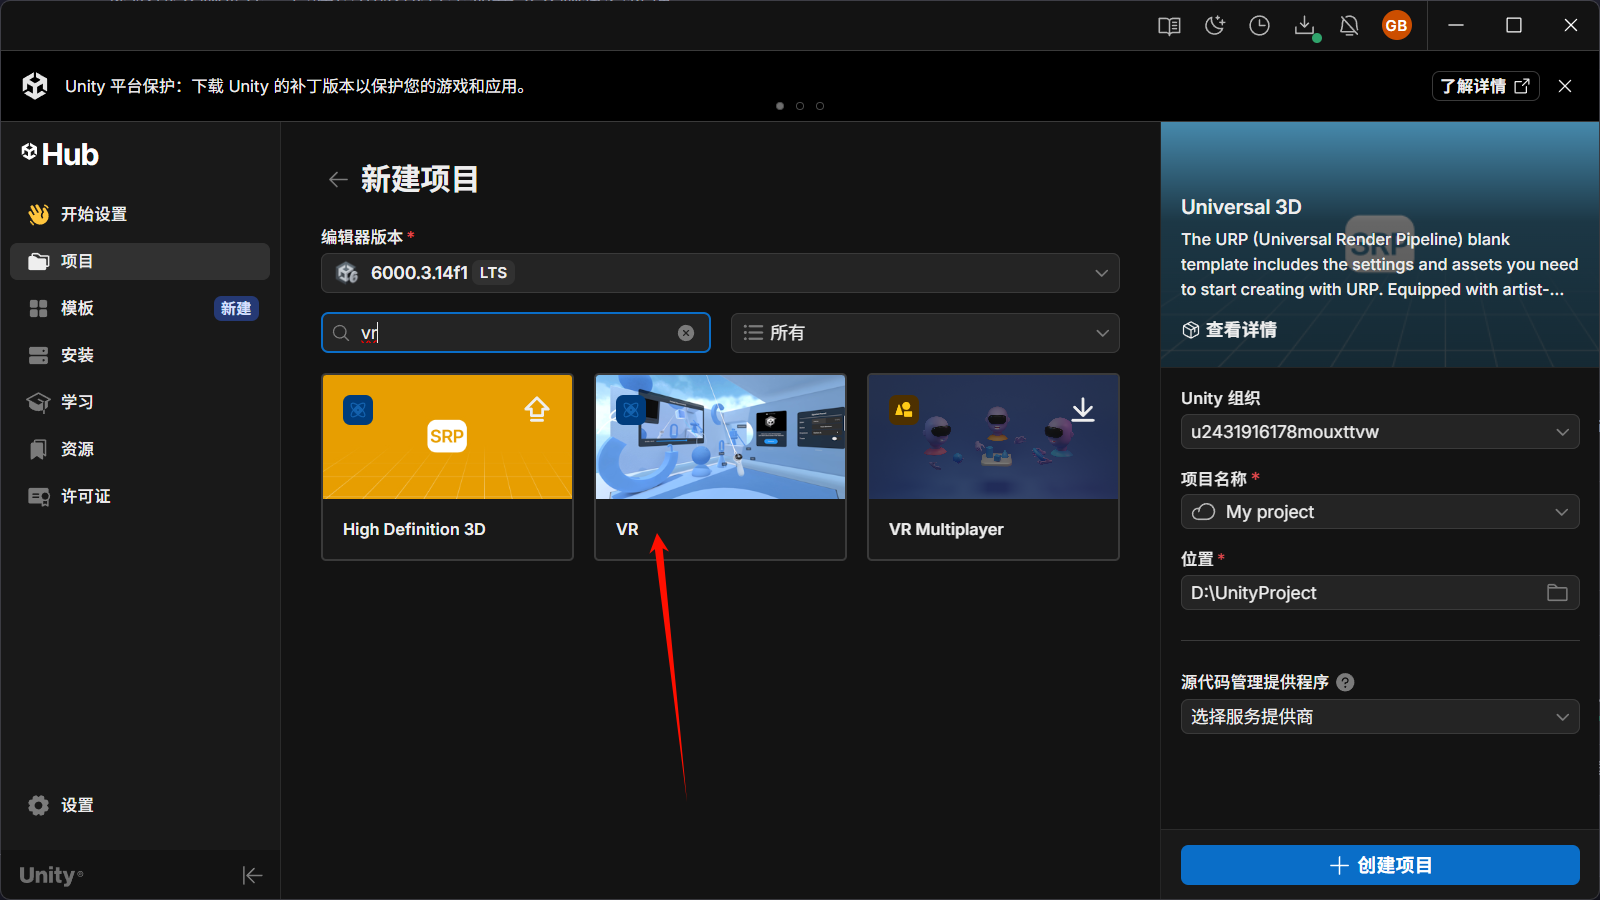
\includegraphics[width=0.86\textwidth]{img/chapter3/创建vr模板.png}
  \caption{创建 Unity VR 模板项目}
  \label{fig:unity_create_vr_template}
\end{figure}

项目创建过程中，Unity 会生成模板场景、默认设置和示例资源。图 \ref{fig:unity_project_creating} 展示了等待项目创建的过程。项目创建完成后进入 Unity 编辑器，能够看到 VR 模板项目的默认场景与资源结构，如图 \ref{fig:unity_enter_project} 所示。

\begin{figure}[htbp]
  \centering
  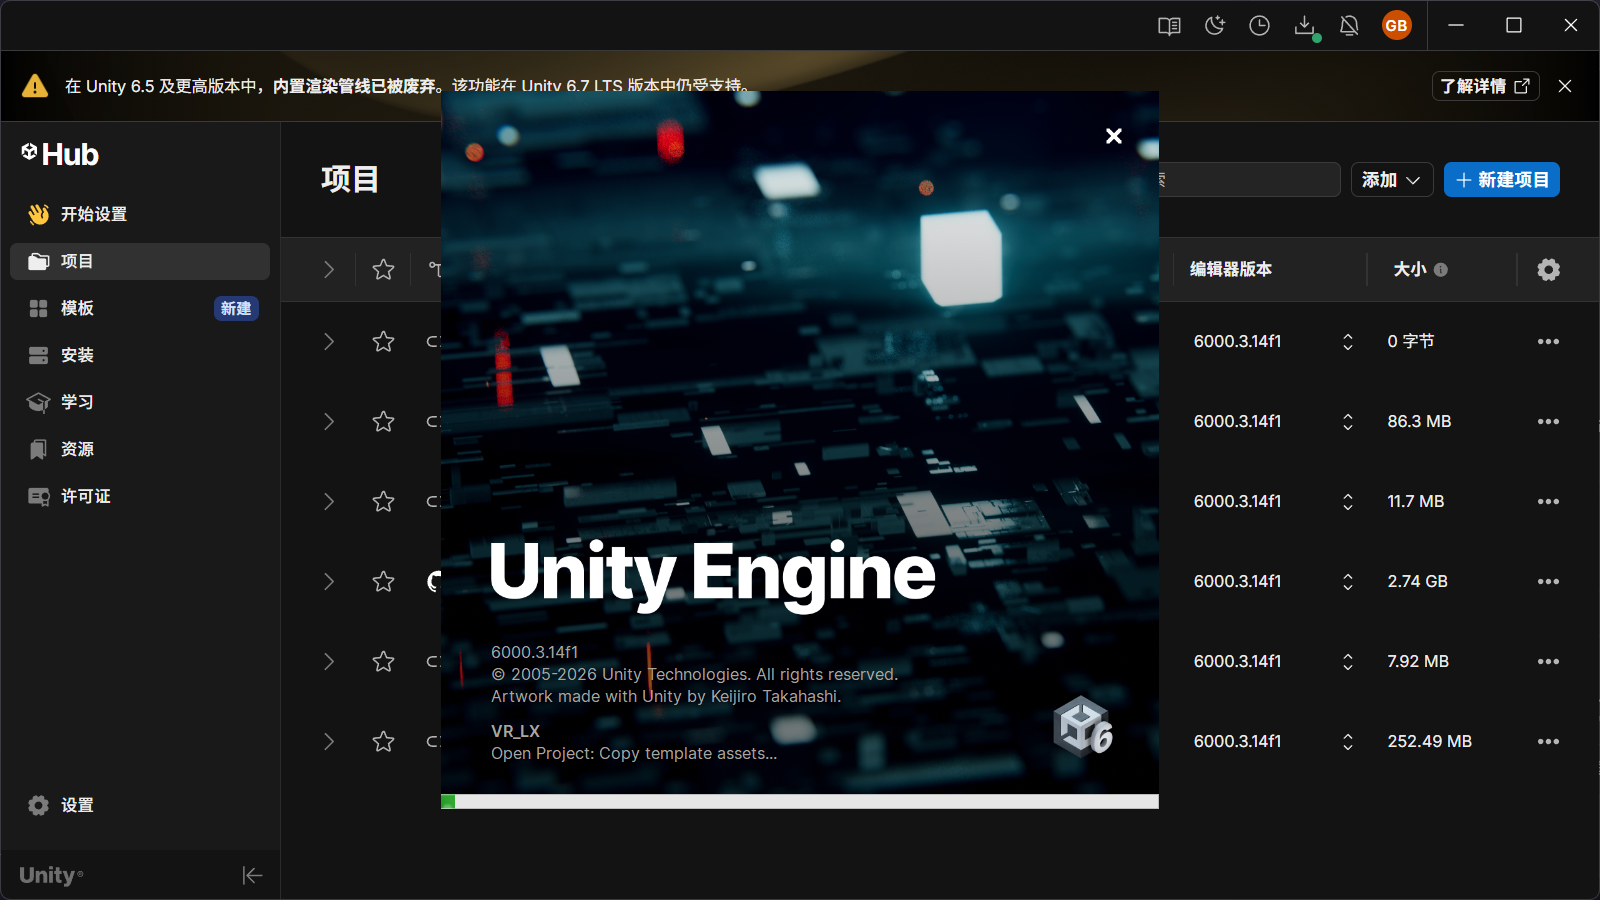
\includegraphics[width=0.86\textwidth]{img/chapter3/等待项目创建.png}
  \caption{Unity VR 项目创建过程}
  \label{fig:unity_project_creating}
\end{figure}

\begin{figure}[htbp]
  \centering
  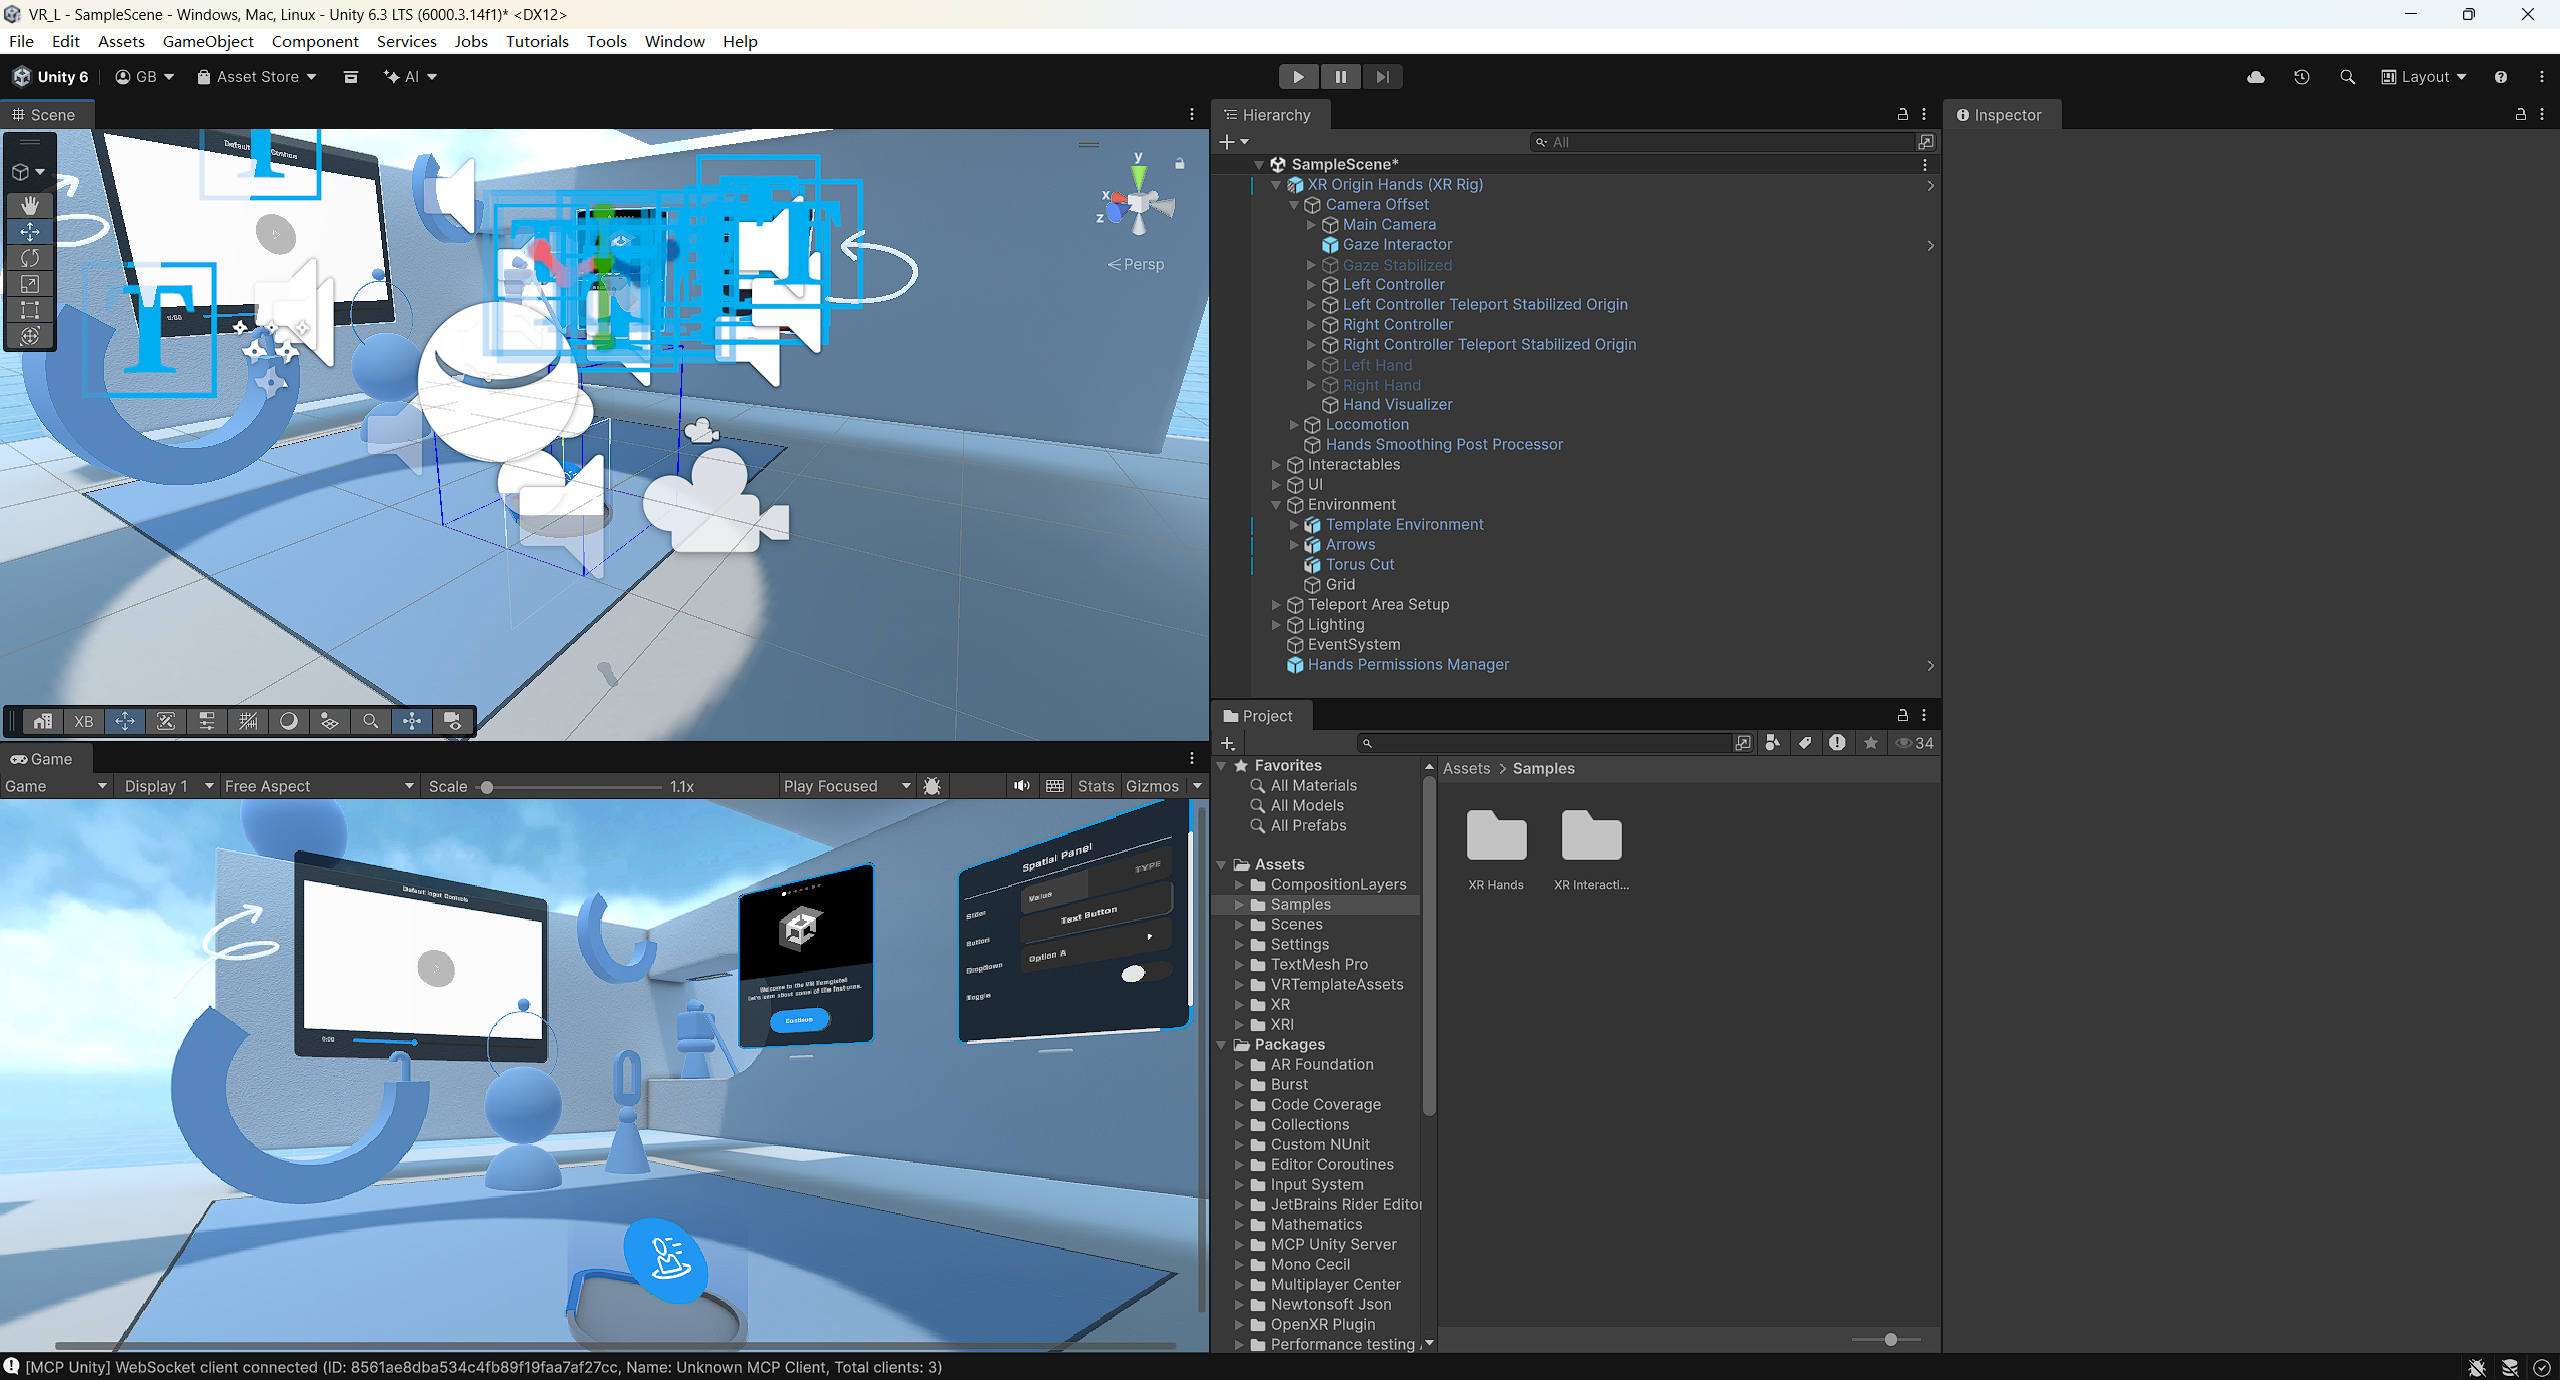
\includegraphics[width=0.86\textwidth]{img/chapter3/进入项目.png}
  \caption{进入 Unity VR 模板项目}
  \label{fig:unity_enter_project}
\end{figure}

\subsubsection{项目环境确认}

为了判断后续导入的场景资源是否兼容，需要先确认当前 Unity 项目版本和渲染管线。本实验项目使用的 Unity 版本为 \mintinline{text}|6000.3.14f1|，渲染管线为 Universal Render Pipeline，URP 包版本为 \mintinline{text}|17.3.0|。其中，Unity 版本可从 \mintinline{text}|ProjectSettings/ProjectVersion.txt| 确认，URP 包版本可从 \mintinline{text}|Packages/manifest.json| 确认，当前渲染管线配置可从 \mintinline{text}|ProjectSettings/GraphicsSettings.asset| 和 URP 配置资产中确认。

这些信息对后续问题定位非常重要。Unity 资源包往往会标注推荐版本和适配的渲染管线。如果资源包面向旧版 Built-in Render Pipeline，而当前项目使用 URP，则材质、Shader 和光照表现可能出现不兼容。实验中出现的粉色材质问题，正是由这一版本和渲染管线差异引起的。

\subsection{导入森林环境资源}

\subsubsection{从 Asset Store 获取资源}

项目创建完成后，实验进入 Unity Asset Store 查找森林环境资源。本次使用的资源包为 \mintinline{text}|Fantasy Forest Environment Free Sample|。该资源包提供了森林样例场景、地形、树木、草地、材质和贴图等内容，能够较快搭建出具有自然环境特征的 VR 展示空间。

\begin{figure}[htbp]
  \centering
  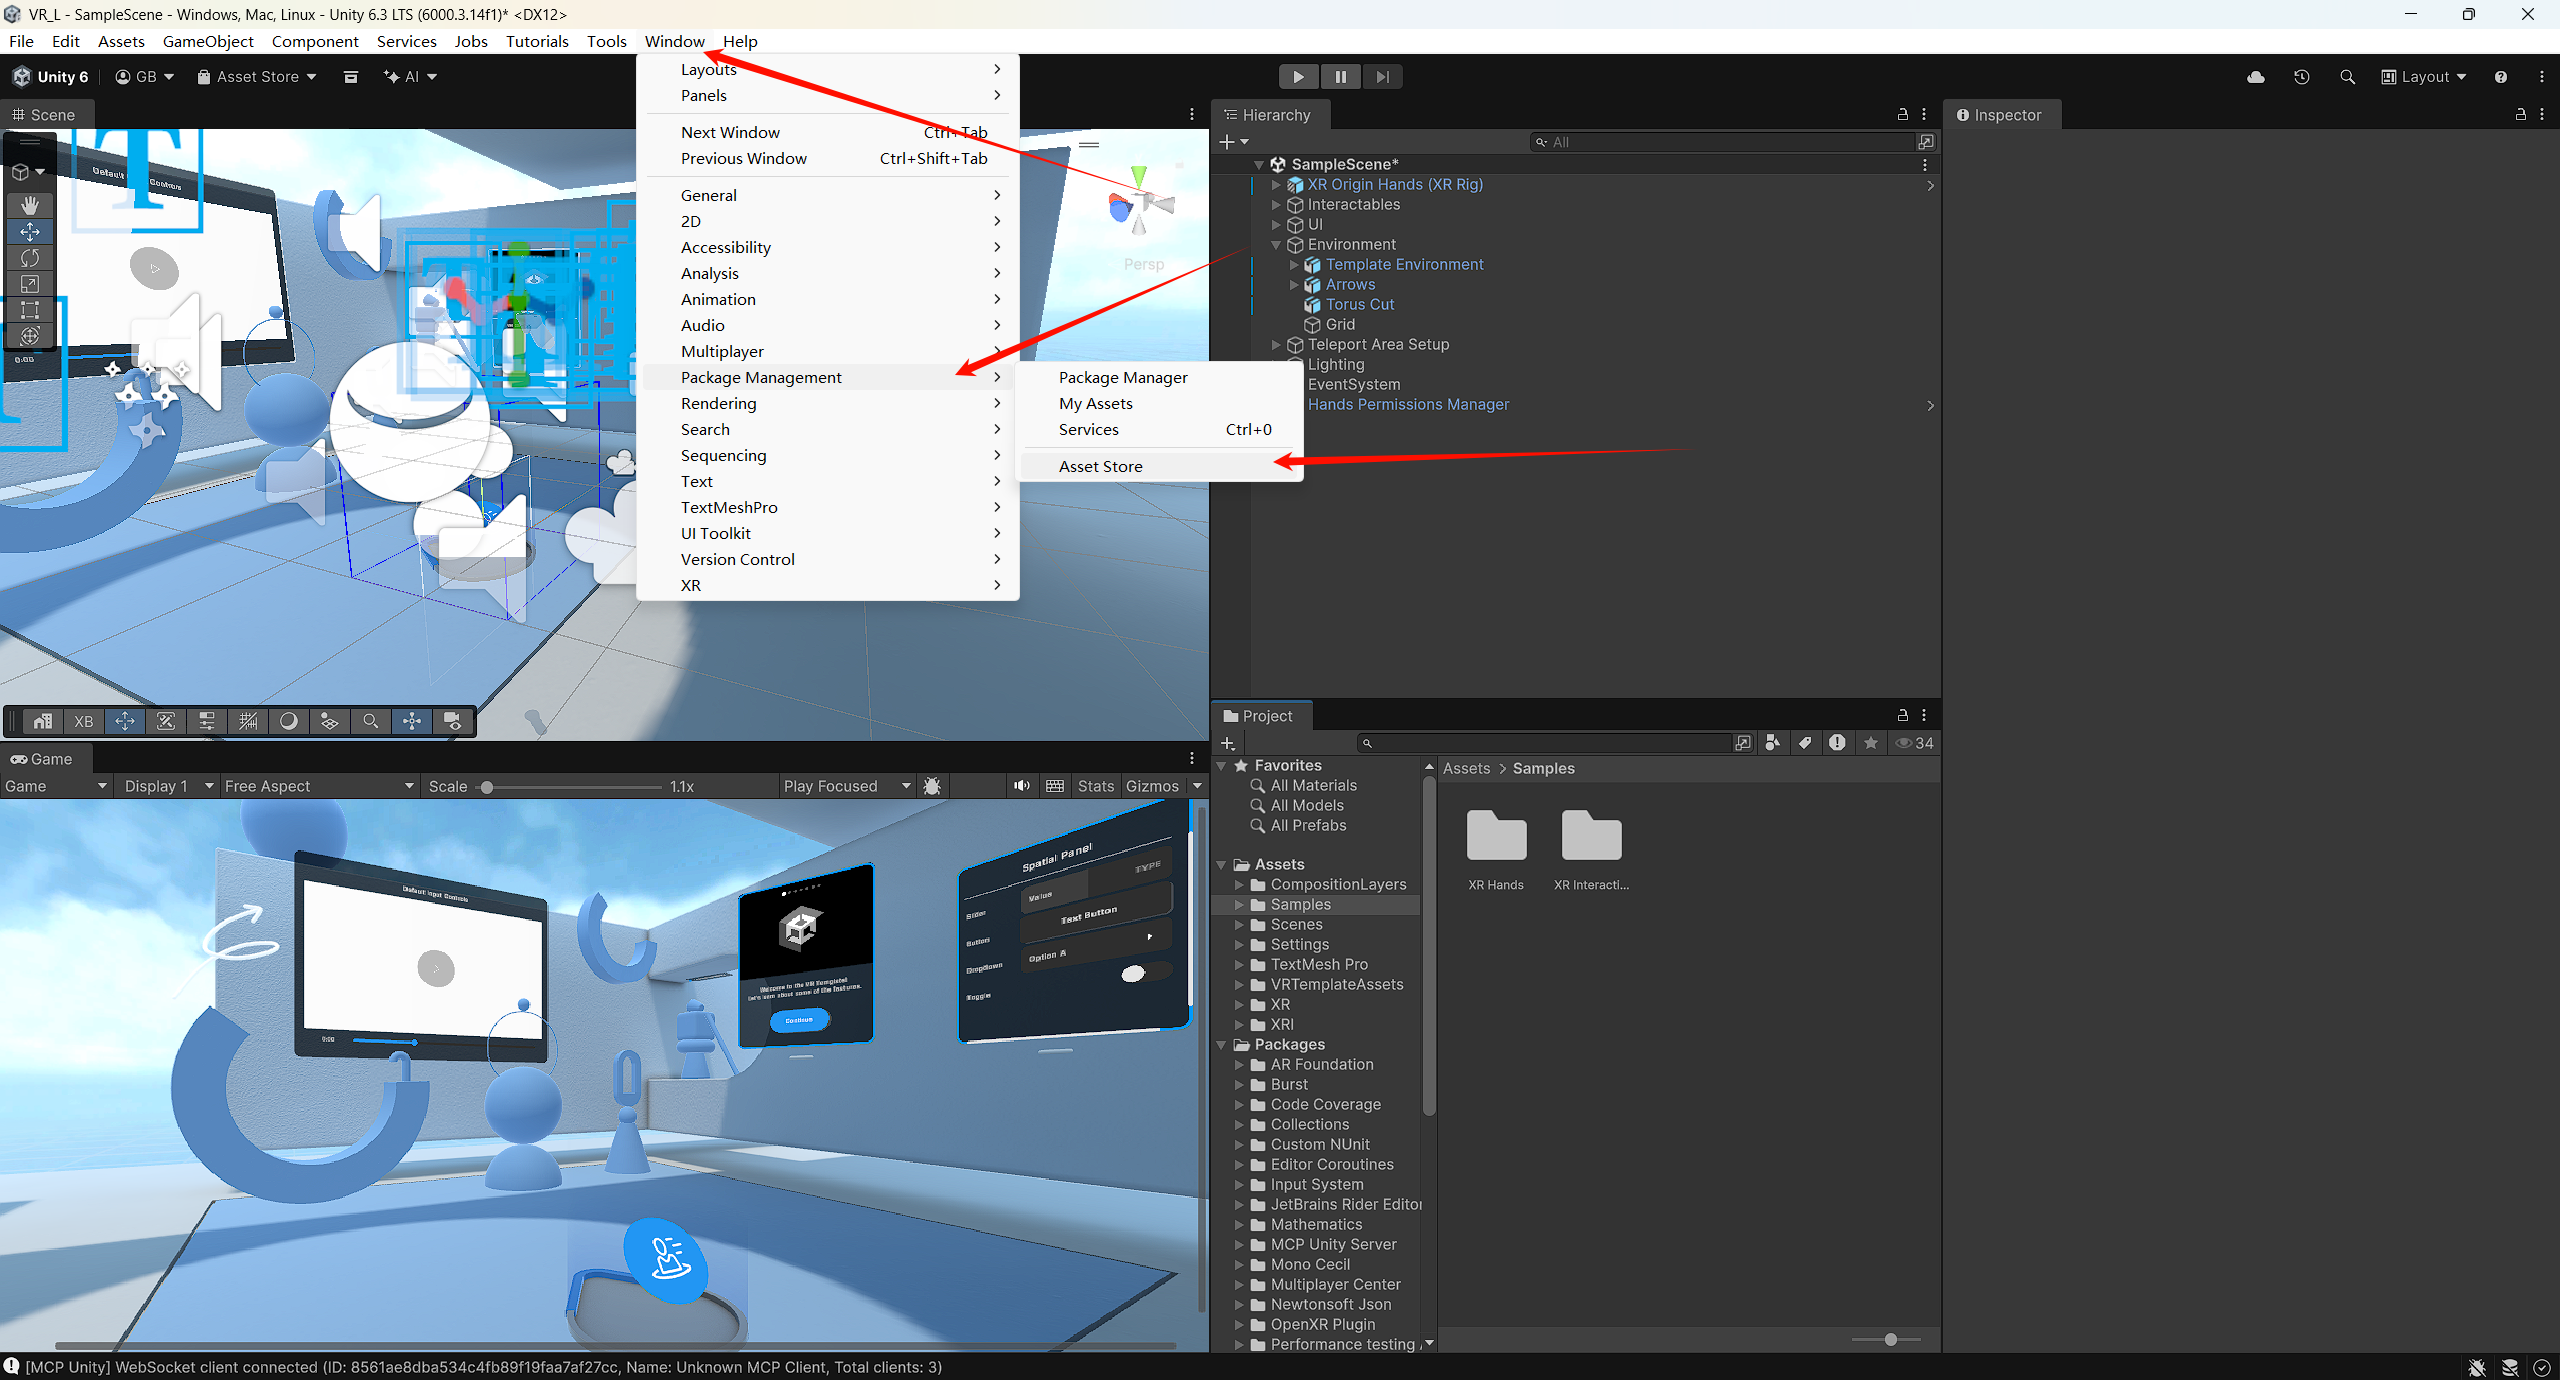
\includegraphics[width=0.86\textwidth]{img/chapter3/前往assetstore.png}
  \caption{在 Unity 中前往 Asset Store}
  \label{fig:unity_go_asset_store}
\end{figure}

\begin{figure}[htbp]
  \centering
  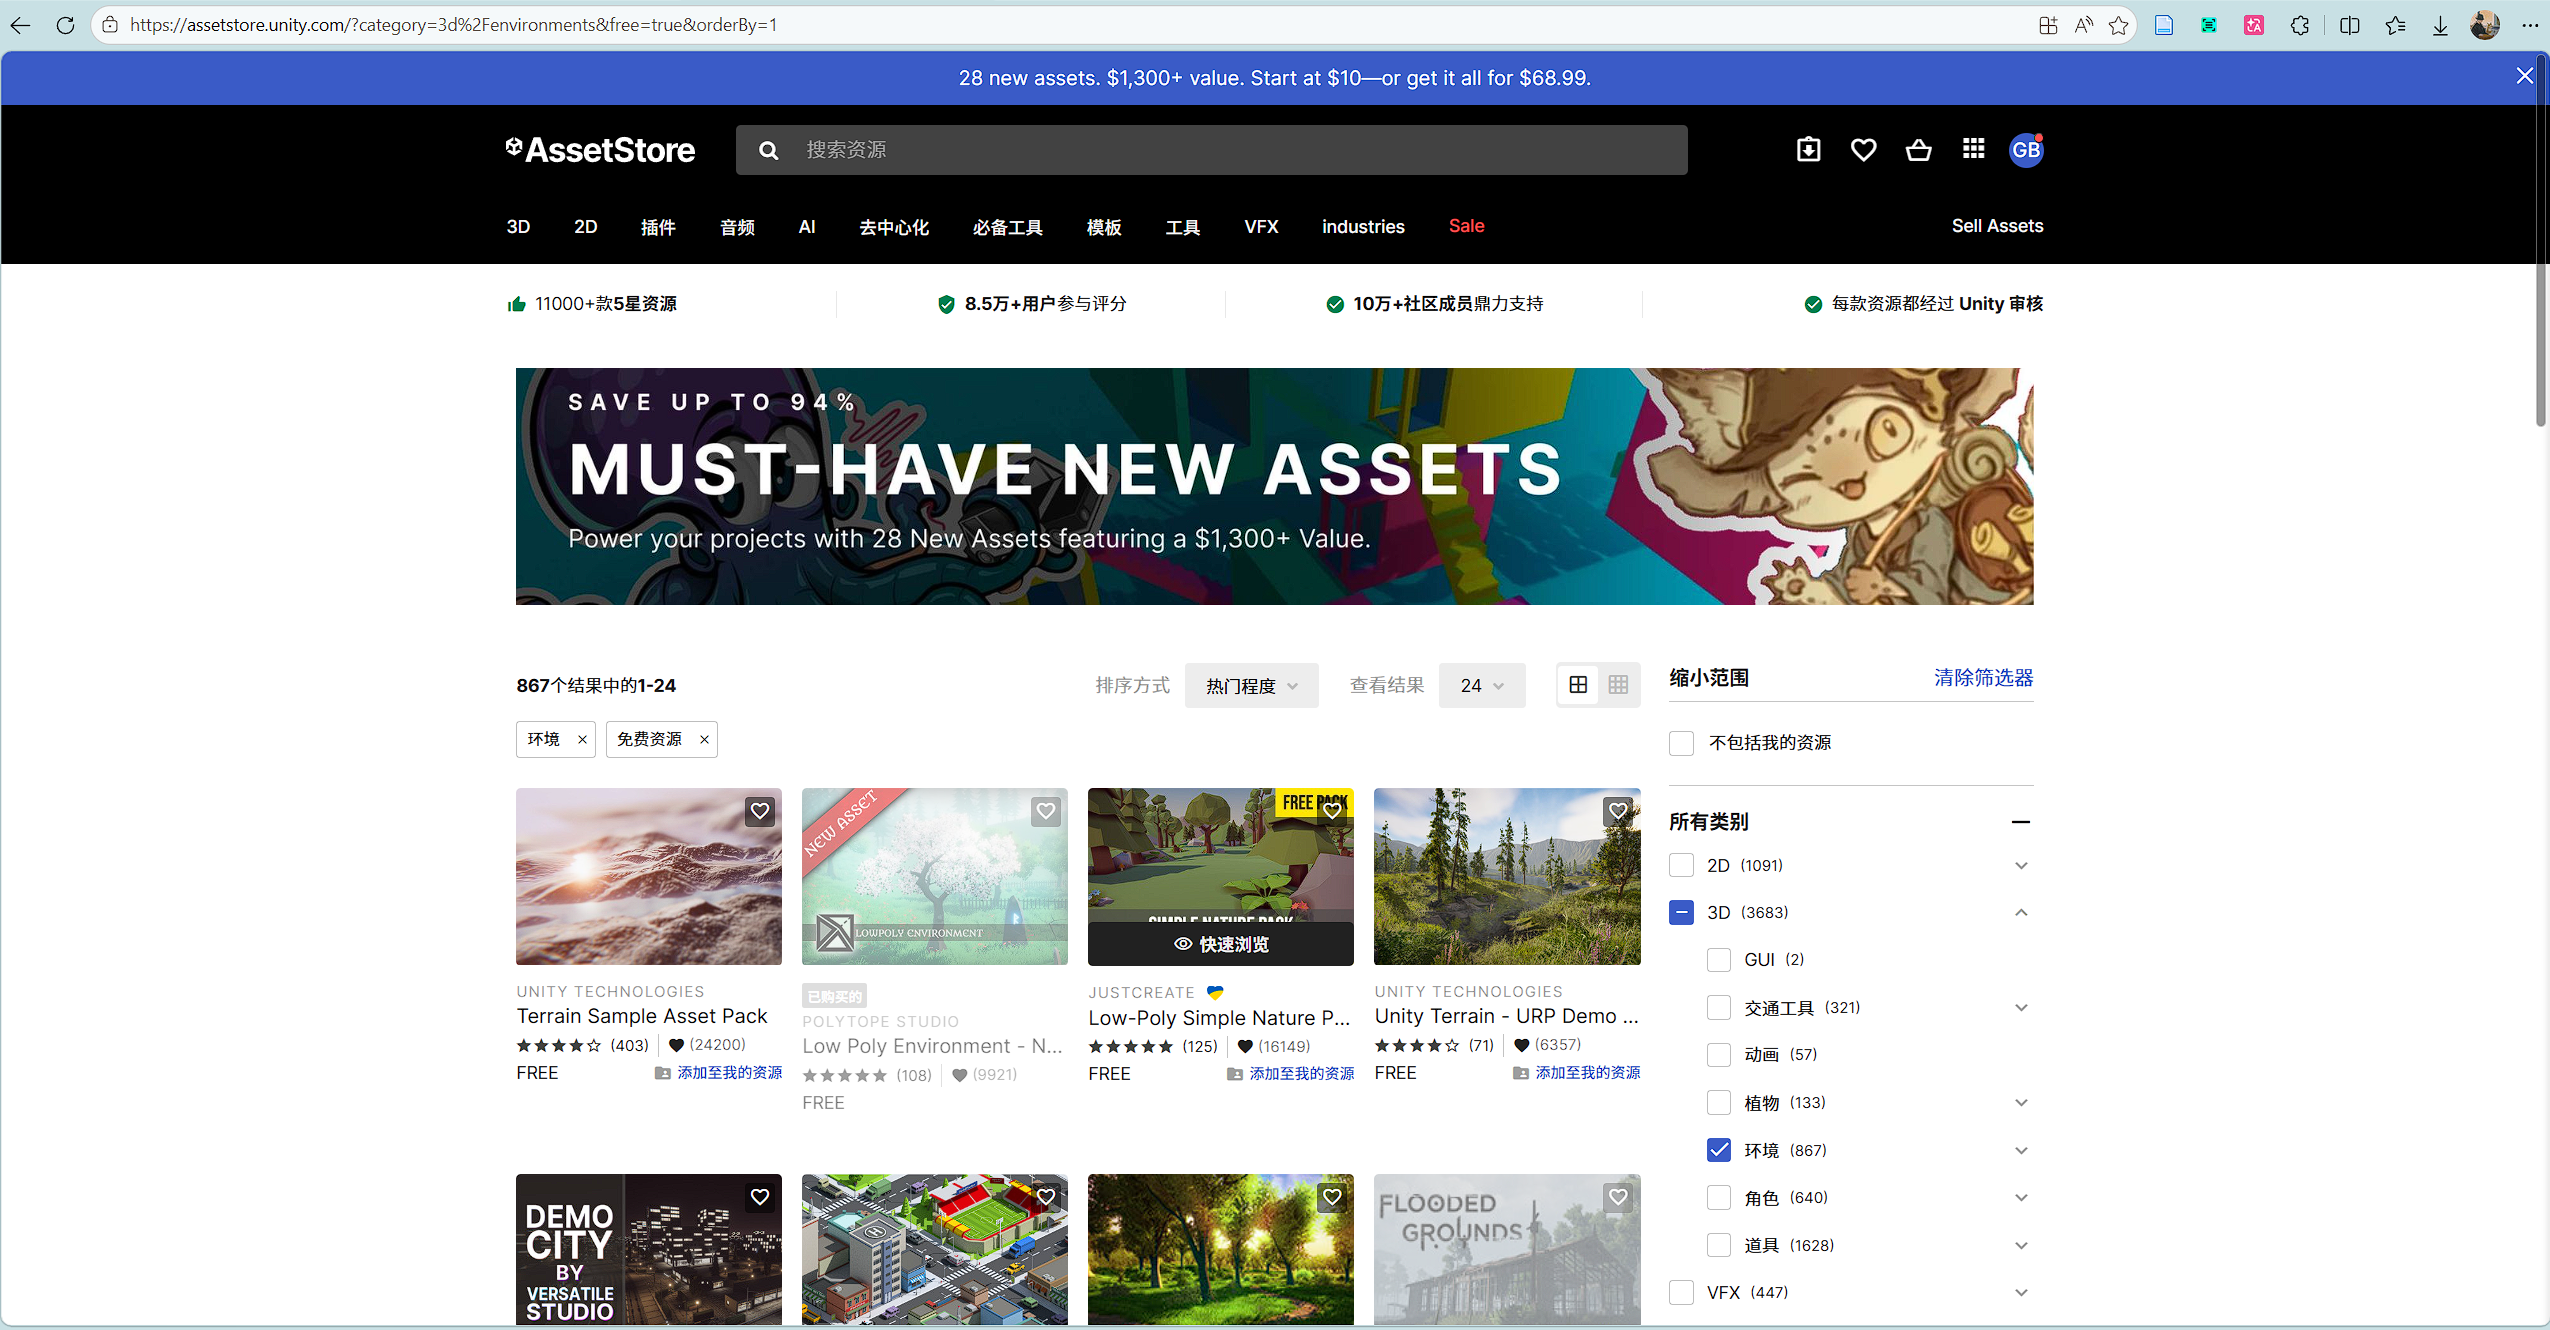
\includegraphics[width=0.86\textwidth]{img/chapter3/AssetStore界面.png}
  \caption{Asset Store 中的森林环境资源}
  \label{fig:unity_asset_store_page}
\end{figure}

资源导入后，项目中新增了 \mintinline{text}|Assets/Fantasy Forest Environment Free Sample| 目录。该目录包含样例场景、材质、模型和资源包自带的 Shader 文件。导入过程如图 \ref{fig:unity_import_forest_asset} 所示。

\begin{figure}[htbp]
  \centering
  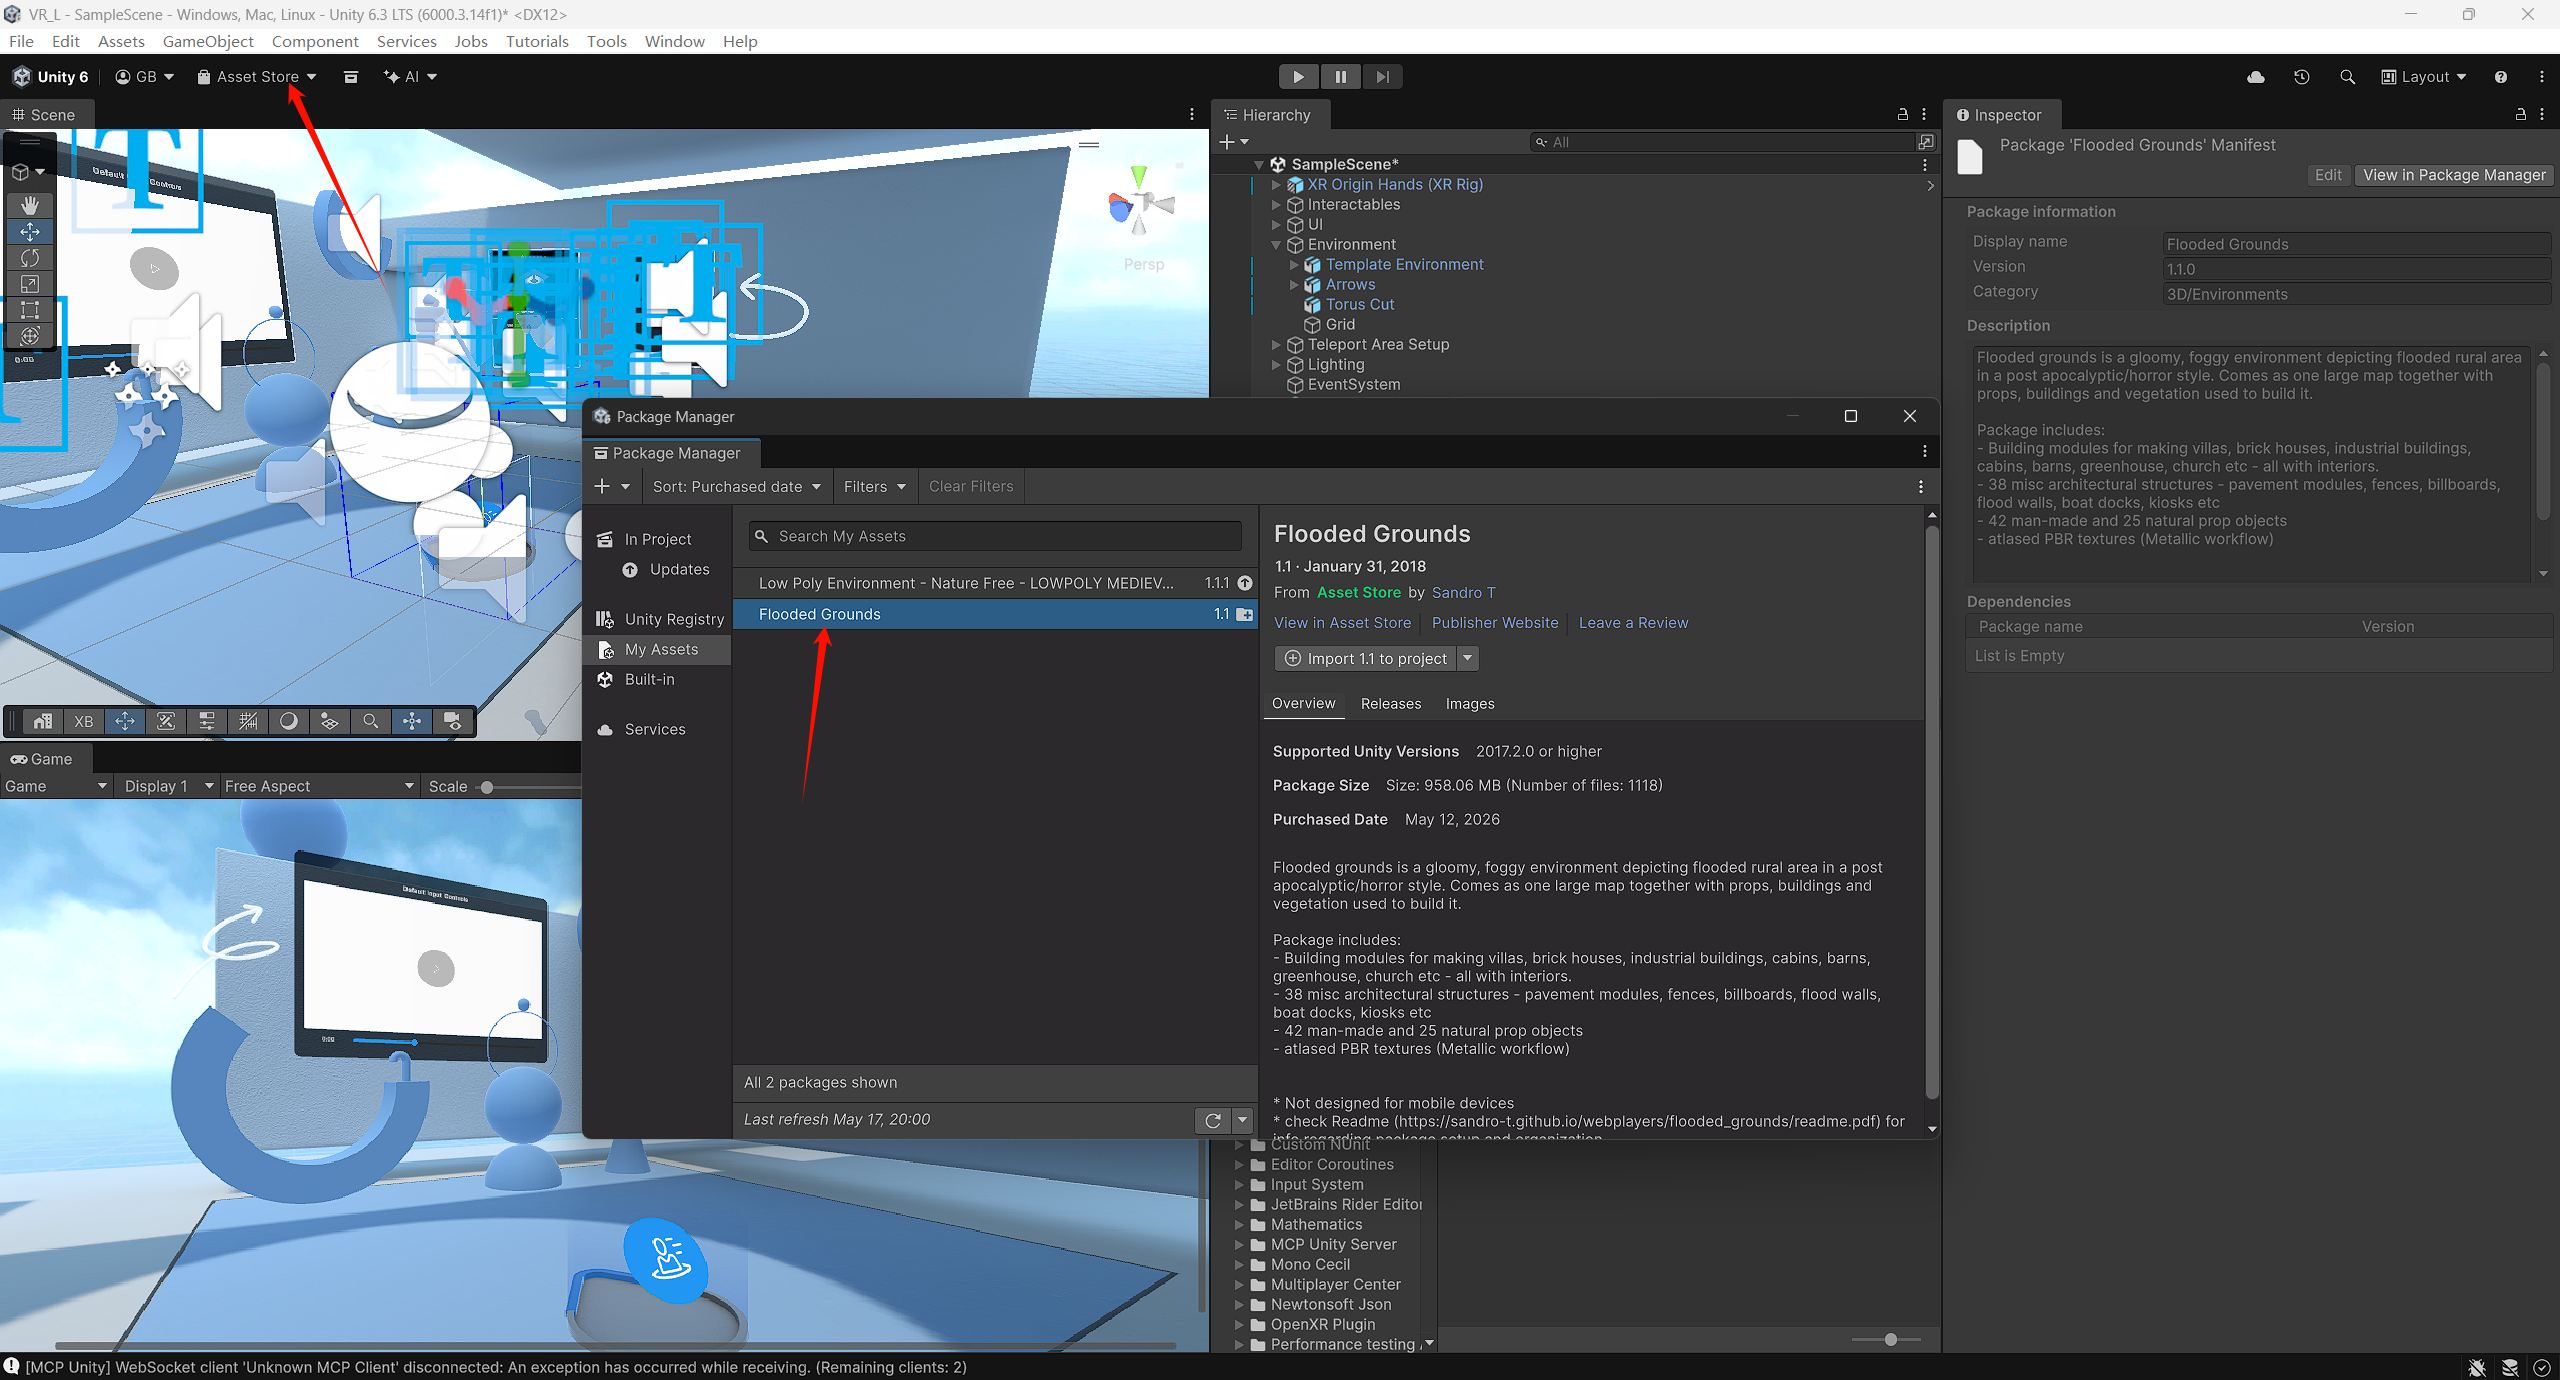
\includegraphics[width=0.86\textwidth]{img/chapter3/导入下载的环境.png}
  \caption{导入 Fantasy Forest Environment Free Sample 资源包}
  \label{fig:unity_import_forest_asset}
\end{figure}

\subsubsection{打开森林样例场景}

资源导入完成后，打开资源包提供的样例场景 \mintinline{text}|Assets/Fantasy Forest Environment Free Sample/Scenes/demoScene_free.unity|。该场景已经包含地形、树木、草地和默认相机，理论上可以直接作为森林环境的展示基础。

但是在当前 Unity 6 + URP 项目中打开样例场景后，模型和材质大面积显示为粉色，如图 \ref{fig:unity_forest_pink} 所示。Unity 中物体显示为粉色，通常表示材质引用的 Shader 无法在当前渲染环境中正常编译或使用。也就是说，场景资源已经导入，但渲染管线不兼容导致它无法正确显示。

\begin{figure}[htbp]
  \centering
  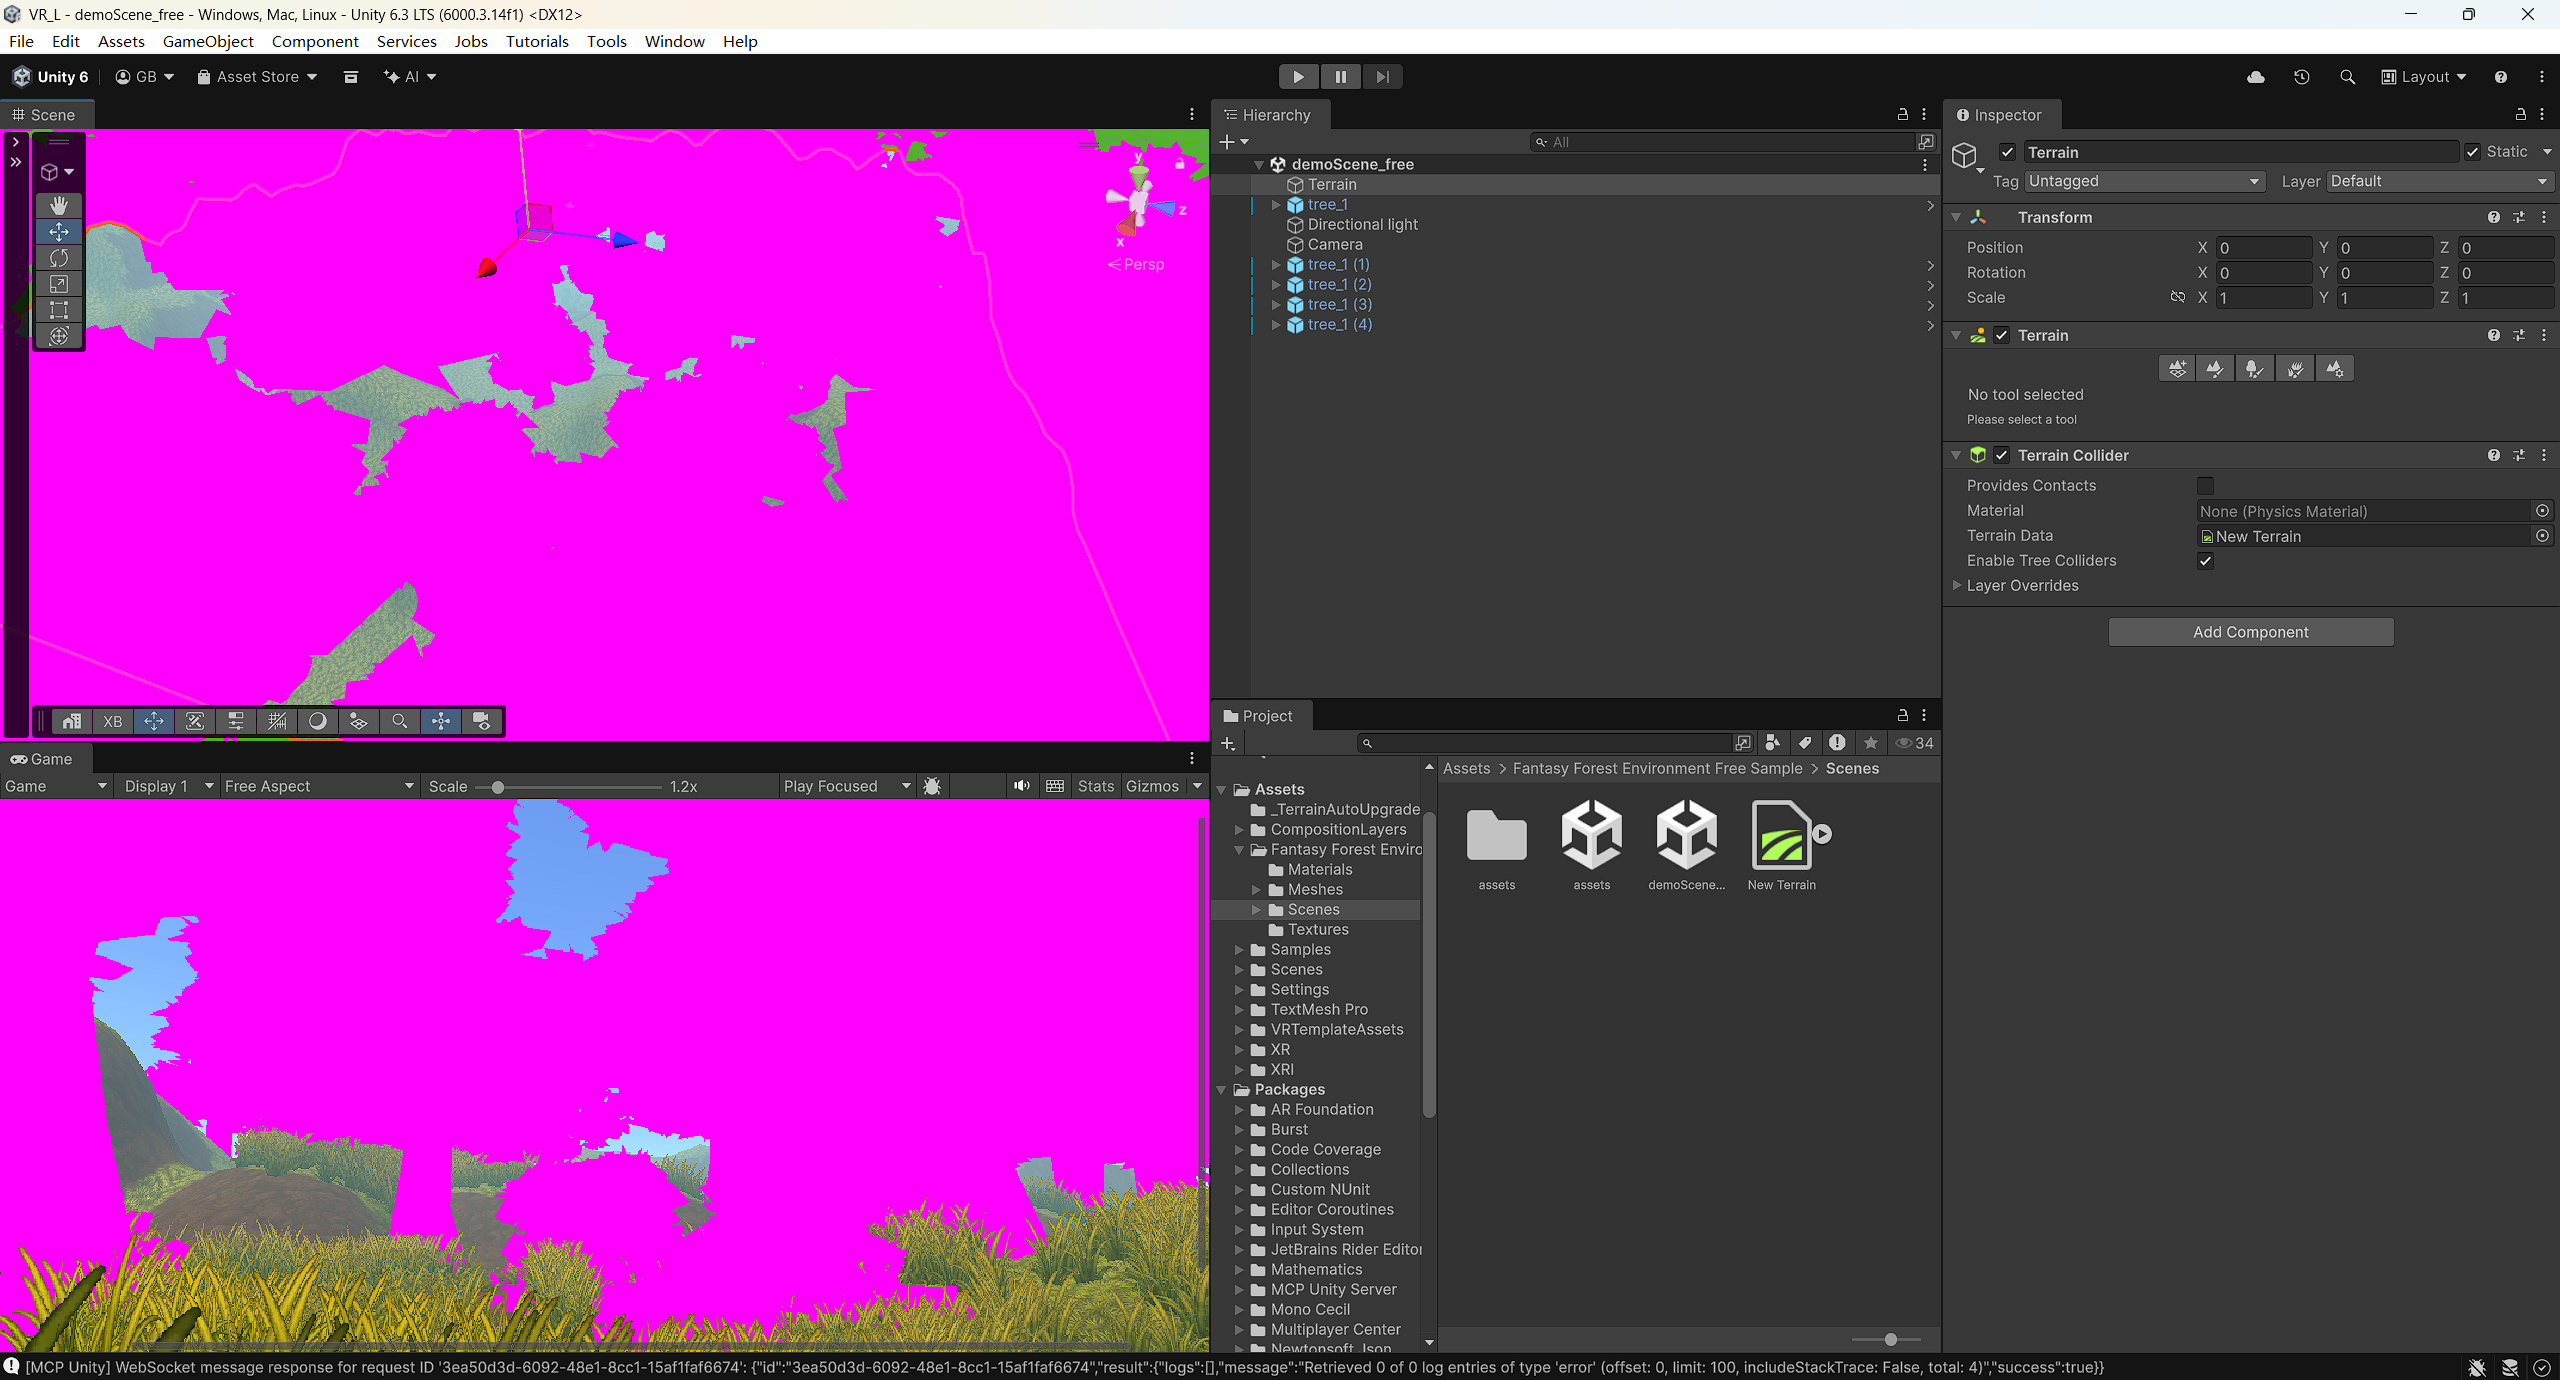
\includegraphics[width=0.86\textwidth]{img/chapter3/打开模板场景冒粉色.png}
  \caption{森林样例场景出现粉色材质}
  \label{fig:unity_forest_pink}
\end{figure}

\subsection{粉色材质问题分析}

\subsubsection{渲染管线不兼容}

检查资源包信息后可以发现，\mintinline{text}|Fantasy Forest Environment Free Sample| 资源包推荐的 Unity 版本为 \mintinline{text}|2021.3.9f1|，资源本身主要面向旧的 Built-in Render Pipeline。而当前实验项目使用 Unity 6 和 URP 17.3.0。Built-in 管线和 URP 在 Shader 写法、光照函数、渲染标签和材质兼容性方面存在差异，因此旧资源包中的 Shader 不能直接在 URP 项目中稳定使用。

进一步检查材质文件后发现，\mintinline{text}|dirt01.mat|、\mintinline{text}|grass01.mat| 等材质仍引用旧的内置 Shader；\mintinline{text}|grassmesh.mat|、\mintinline{text}|tree_branches.mat| 等材质则引用资源包自带的 \mintinline{text}|Fantasy Forest/StandardNoCulling| Shader。原始 \mintinline{text}|StandardNoCulling.shader| 使用 Built-in 管线的 Surface Shader 写法，例如 \mintinline{text}|#pragma surface surf StandardSpecular|。URP 不支持这种 Built-in Surface Shader，因此这些材质在当前项目中无法正常渲染。

\subsubsection{植被材质的特殊要求}

森林资源中的草、树叶和树枝并不是普通不透明模型。为了让草片和树叶从正反两面都可见，材质需要保留双面显示逻辑；为了让贴图中透明区域不遮挡背景，材质还需要使用透明裁剪；为了让场景具备空间层次，植被对象还应能参与阴影投射。因此，修复时不能只把材质简单替换为普通 URP Lit Shader，还要保留原资源对双面渲染和 alpha 裁剪的需求。

基于这一判断，本实验没有选择降级 Unity 版本，也没有重新创建 Unity 2021 的 Built-in 项目。当前项目已经包含 VR 模板、URP、XR 和输入系统等依赖，直接降级项目存在较高风险。更合适的方式是在当前 Unity 6 + URP 项目中修复资源包的 Shader 和材质引用，使森林资源适配当前实验环境。

\subsection{URP Shader 修复过程}

\subsubsection{修改 StandardNoCulling Shader}

本次代码级修复集中在资源包自带的 Shader 文件：

\begin{minted}{text}
Assets/Fantasy Forest Environment Free Sample/StandardNoCulling.shader
\end{minted}

修复思路是将旧 Built-in Surface Shader 改写为 URP 可用的 HLSL Shader，并继续使用原来的 Shader 名称 \mintinline{text}|Fantasy Forest/StandardNoCulling|。这样，已经引用该 Shader 的材质可以自动使用兼容版本，不需要逐个重建材质。

修复后的 Shader 保留了资源包原本需要的 \mintinline{text}|_MainTex|、\mintinline{text}|_Color|、\mintinline{text}|_Cutoff| 和 \mintinline{text}|_Glossiness| 属性。其中，\mintinline{text}|_MainTex| 用于基础贴图，\mintinline{text}|_Color| 用于颜色叠加，\mintinline{text}|_Cutoff| 用于透明裁剪阈值，\mintinline{text}|_Glossiness| 用于控制光滑度。SubShader 中增加 \mintinline{text}|RenderPipeline = UniversalPipeline| 标签，明确它面向 URP 使用。

核心渲染通道使用 \mintinline{text}|UniversalForward|，通过 URP 的 \mintinline{text}|Core.hlsl| 和 \mintinline{text}|Lighting.hlsl| 获取顶点变换、法线、主光源、阴影和雾效支持。片元阶段先采样基础贴图，并通过贴图 alpha 执行透明裁剪，再构造 \mintinline{text}|InputData| 与 \mintinline{text}|SurfaceData|，最后调用 \mintinline{text}|UniversalFragmentPBR| 输出光照结果。这样可以让草地、树叶和树干在 URP 中获得基本的 PBR 光照表现。

\subsubsection{保留双面渲染和阴影}

森林植被资源需要从正反两面都能看到，因此 Shader 中保留了 \mintinline{text}|Cull Off|。如果开启背面剔除，草片或树叶从背面观察时可能直接消失，VR 场景中的沉浸感会明显下降。对于森林这种视角自由移动的场景，双面渲染比普通静态截图更重要。

同时，修复后的 Shader 增加了 \mintinline{text}|ShadowCaster| pass。该 pass 使用同样的贴图 alpha 裁剪逻辑，使草、树叶等带透明区域的模型能够以正确轮廓参与阴影计算。否则，即使物体本身能够显示，也可能出现阴影缺失或阴影形状不合理的问题。

值得注意的是，本次透明裁剪使用贴图 alpha，而不是直接使用 \mintinline{text}|_Color.a|。这是因为原资源中部分树叶材质的颜色 alpha 可能为 0，如果直接按 \mintinline{text}|_Color.a| 裁剪，会把树叶错误裁掉。改为依据贴图 alpha 判断，可以更符合资源原本的透明区域设计。

\subsubsection{调整材质引用}

Shader 修复完成后，还需要让相关材质引用新的兼容 Shader。实验中将以下材质统一改为引用 \mintinline{text}|Fantasy Forest/StandardNoCulling|：

\begin{itemize}
  \item \mintinline{text}|Assets/Fantasy Forest Environment Free Sample/Materials/dirt01.mat|
  \item \mintinline{text}|Assets/Fantasy Forest Environment Free Sample/Materials/grass01.mat|
  \item \mintinline{text}|Assets/Fantasy Forest Environment Free Sample/Materials/bark01_bottom.mat|
\end{itemize}

另外，\mintinline{text}|grassmesh.mat| 和 \mintinline{text}|tree_branches.mat| 原本已经引用 \mintinline{text}|Fantasy Forest/StandardNoCulling|，因此在 Shader 文件修复后会自动使用新的 URP 兼容实现。完成修改后，Unity 重新编译通过，Console 中没有 Shader 或脚本编译错误，相关材质能够识别到 \mintinline{text}|Shader: Fantasy Forest/StandardNoCulling|。

\begin{figure}[htbp]
  \centering
  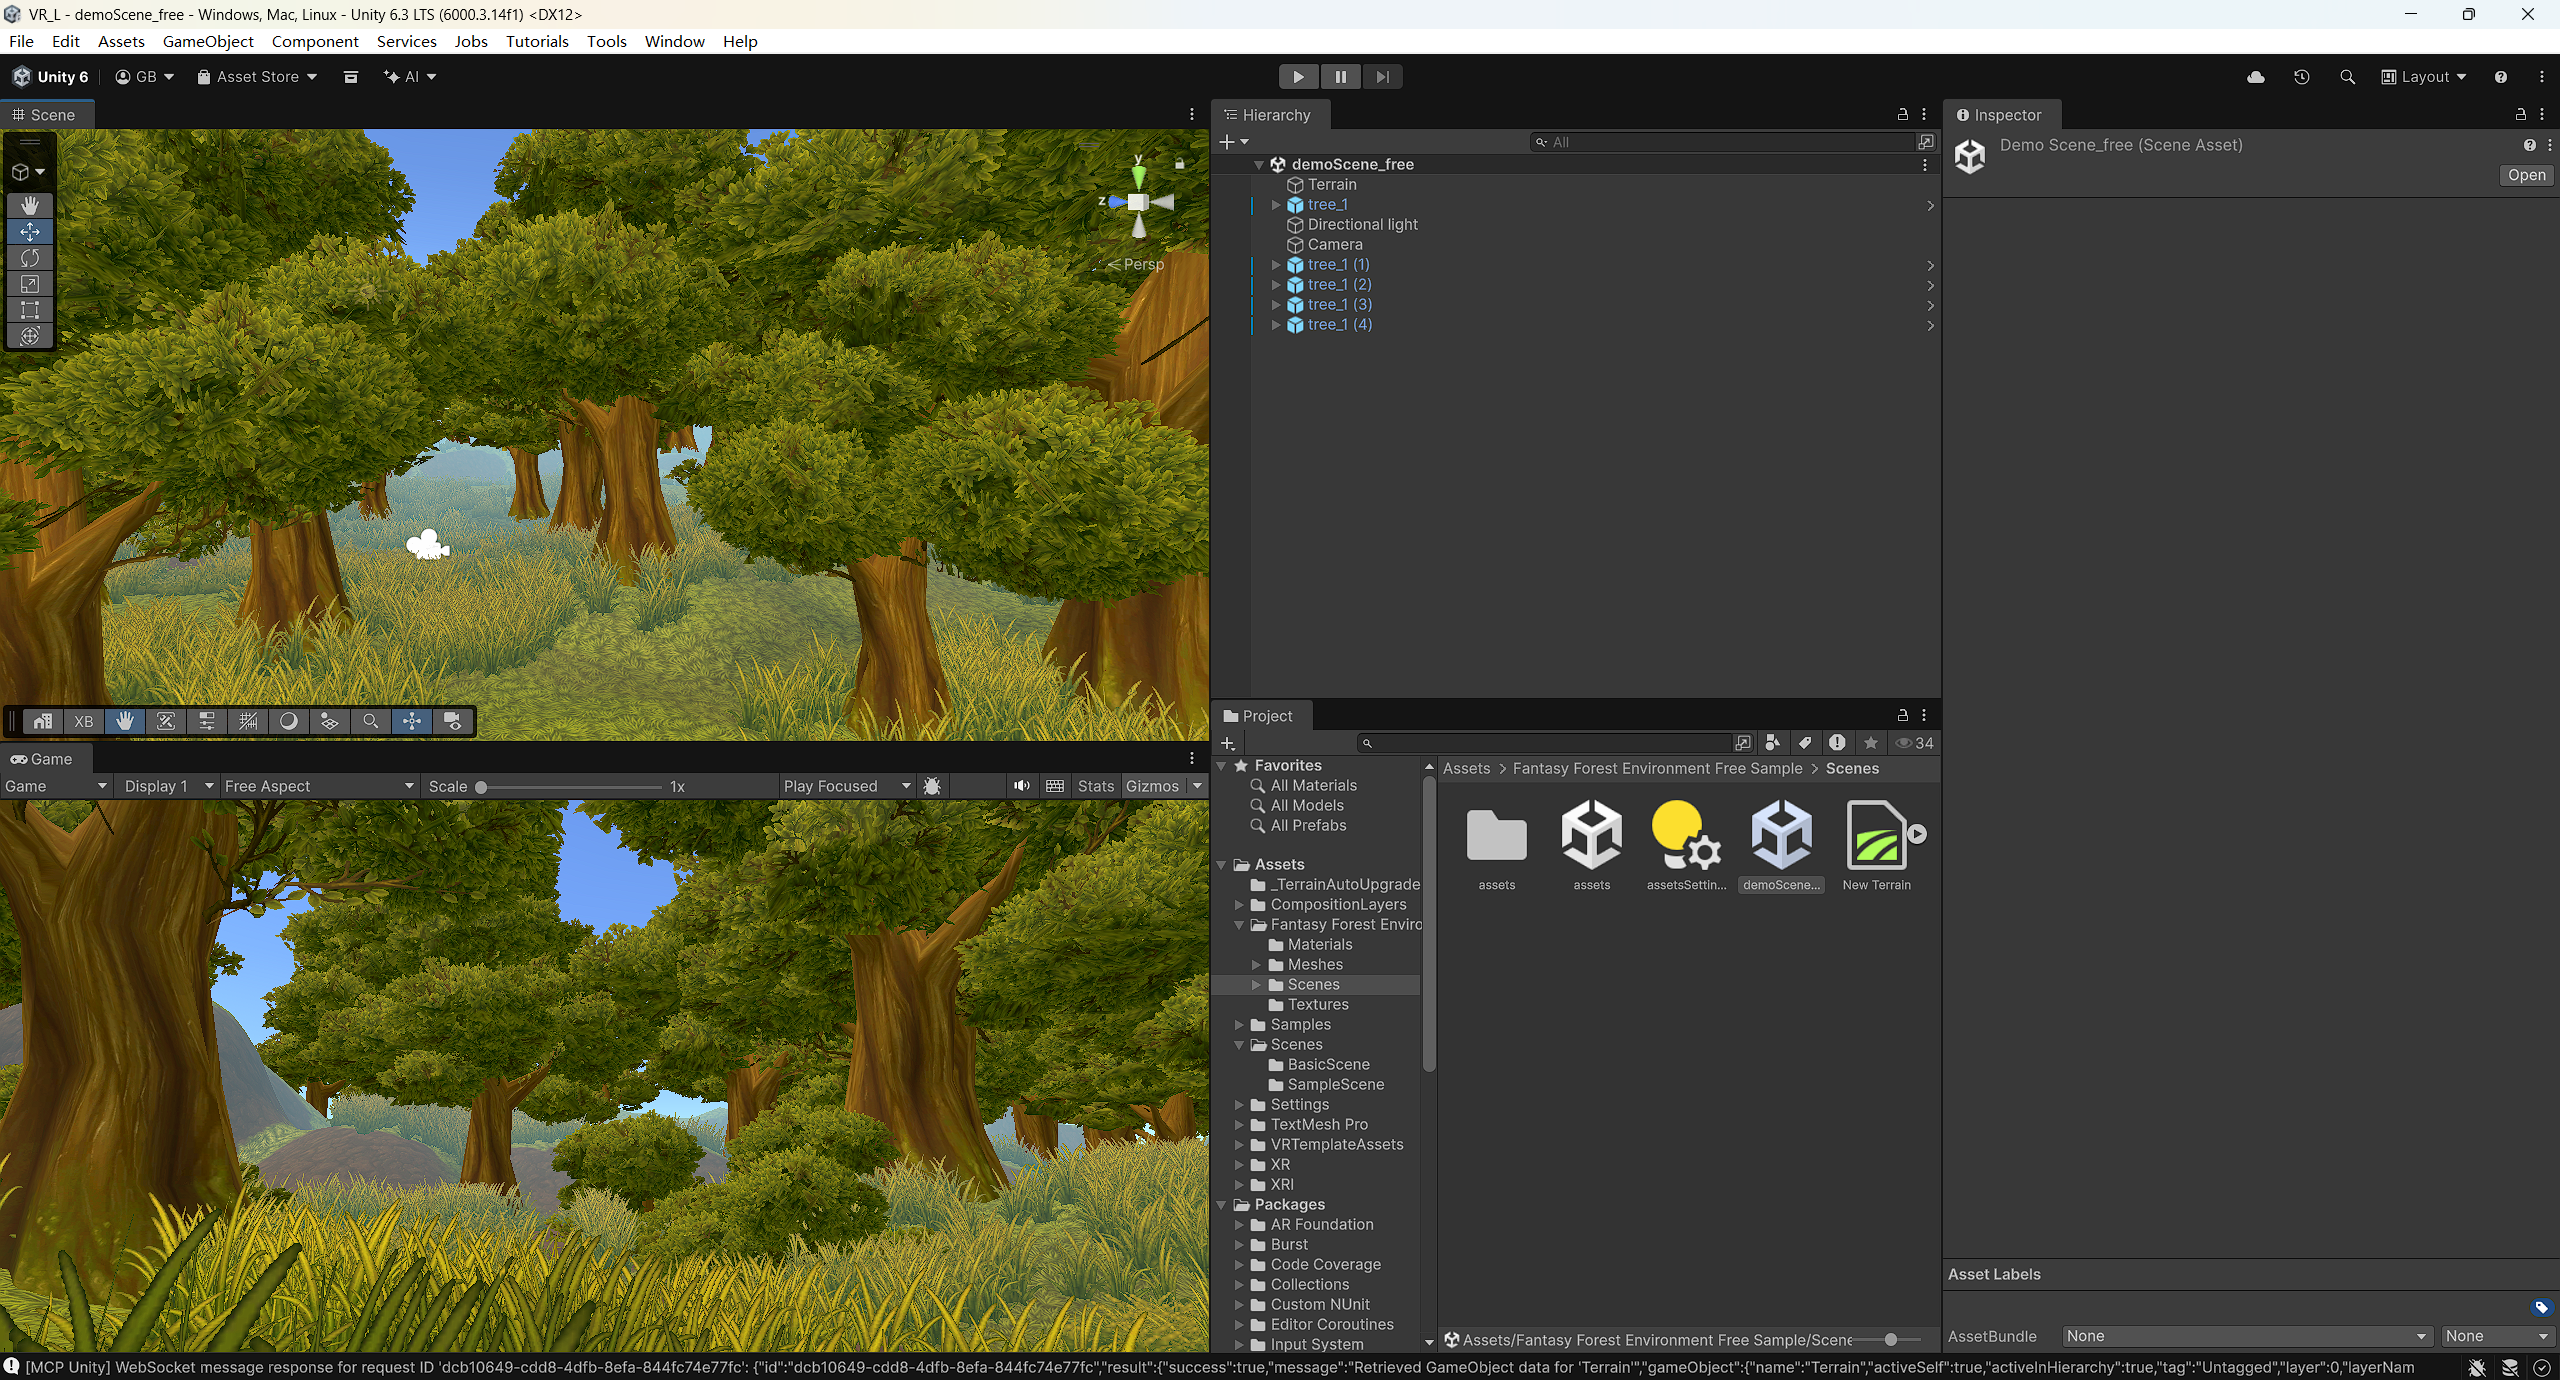
\includegraphics[width=0.86\textwidth]{img/chapter3/修改后正常显示.png}
  \caption{修复 Shader 和材质后森林场景正常显示}
  \label{fig:unity_forest_fixed}
\end{figure}

\subsection{接入 VR 视角}

\subsubsection{复制 XR Origin}

森林样例场景修复后，下一步是把 VR 模板项目中的 VR 视角接入森林场景。这里没有只复制单独的 Camera，而是复制完整的 XR Origin 预制体：

\begin{minted}{text}
Assets/VRTemplateAssets/Prefabs/Setup/Complete XR Origin Set Up Hands Variant.prefab
\end{minted}

这样做的原因是，VR 视角并不只是一个摄像机。完整的 XR Origin 通常包含 \mintinline{text}|Main Camera|、\mintinline{text}|Camera Offset|、手部模型、控制器、输入行为和移动相关组件。如果只复制普通 Camera，场景可能可以显示画面，但无法完整保留 VR 模板中的手部、控制器和交互输入结构。

源场景为 \mintinline{text}|Assets/Scenes/SampleScene.unity|，目标场景为 \mintinline{text}|Assets/Fantasy Forest Environment Free Sample/Scenes/demoScene_free.unity|。实验在目标森林场景中新增 \mintinline{text}|XR Origin Hands (XR Rig)|，并将其位置设置到原普通相机附近，使用户进入 VR 后能够从合适的位置观察森林环境。

\begin{figure}[htbp]
  \centering
  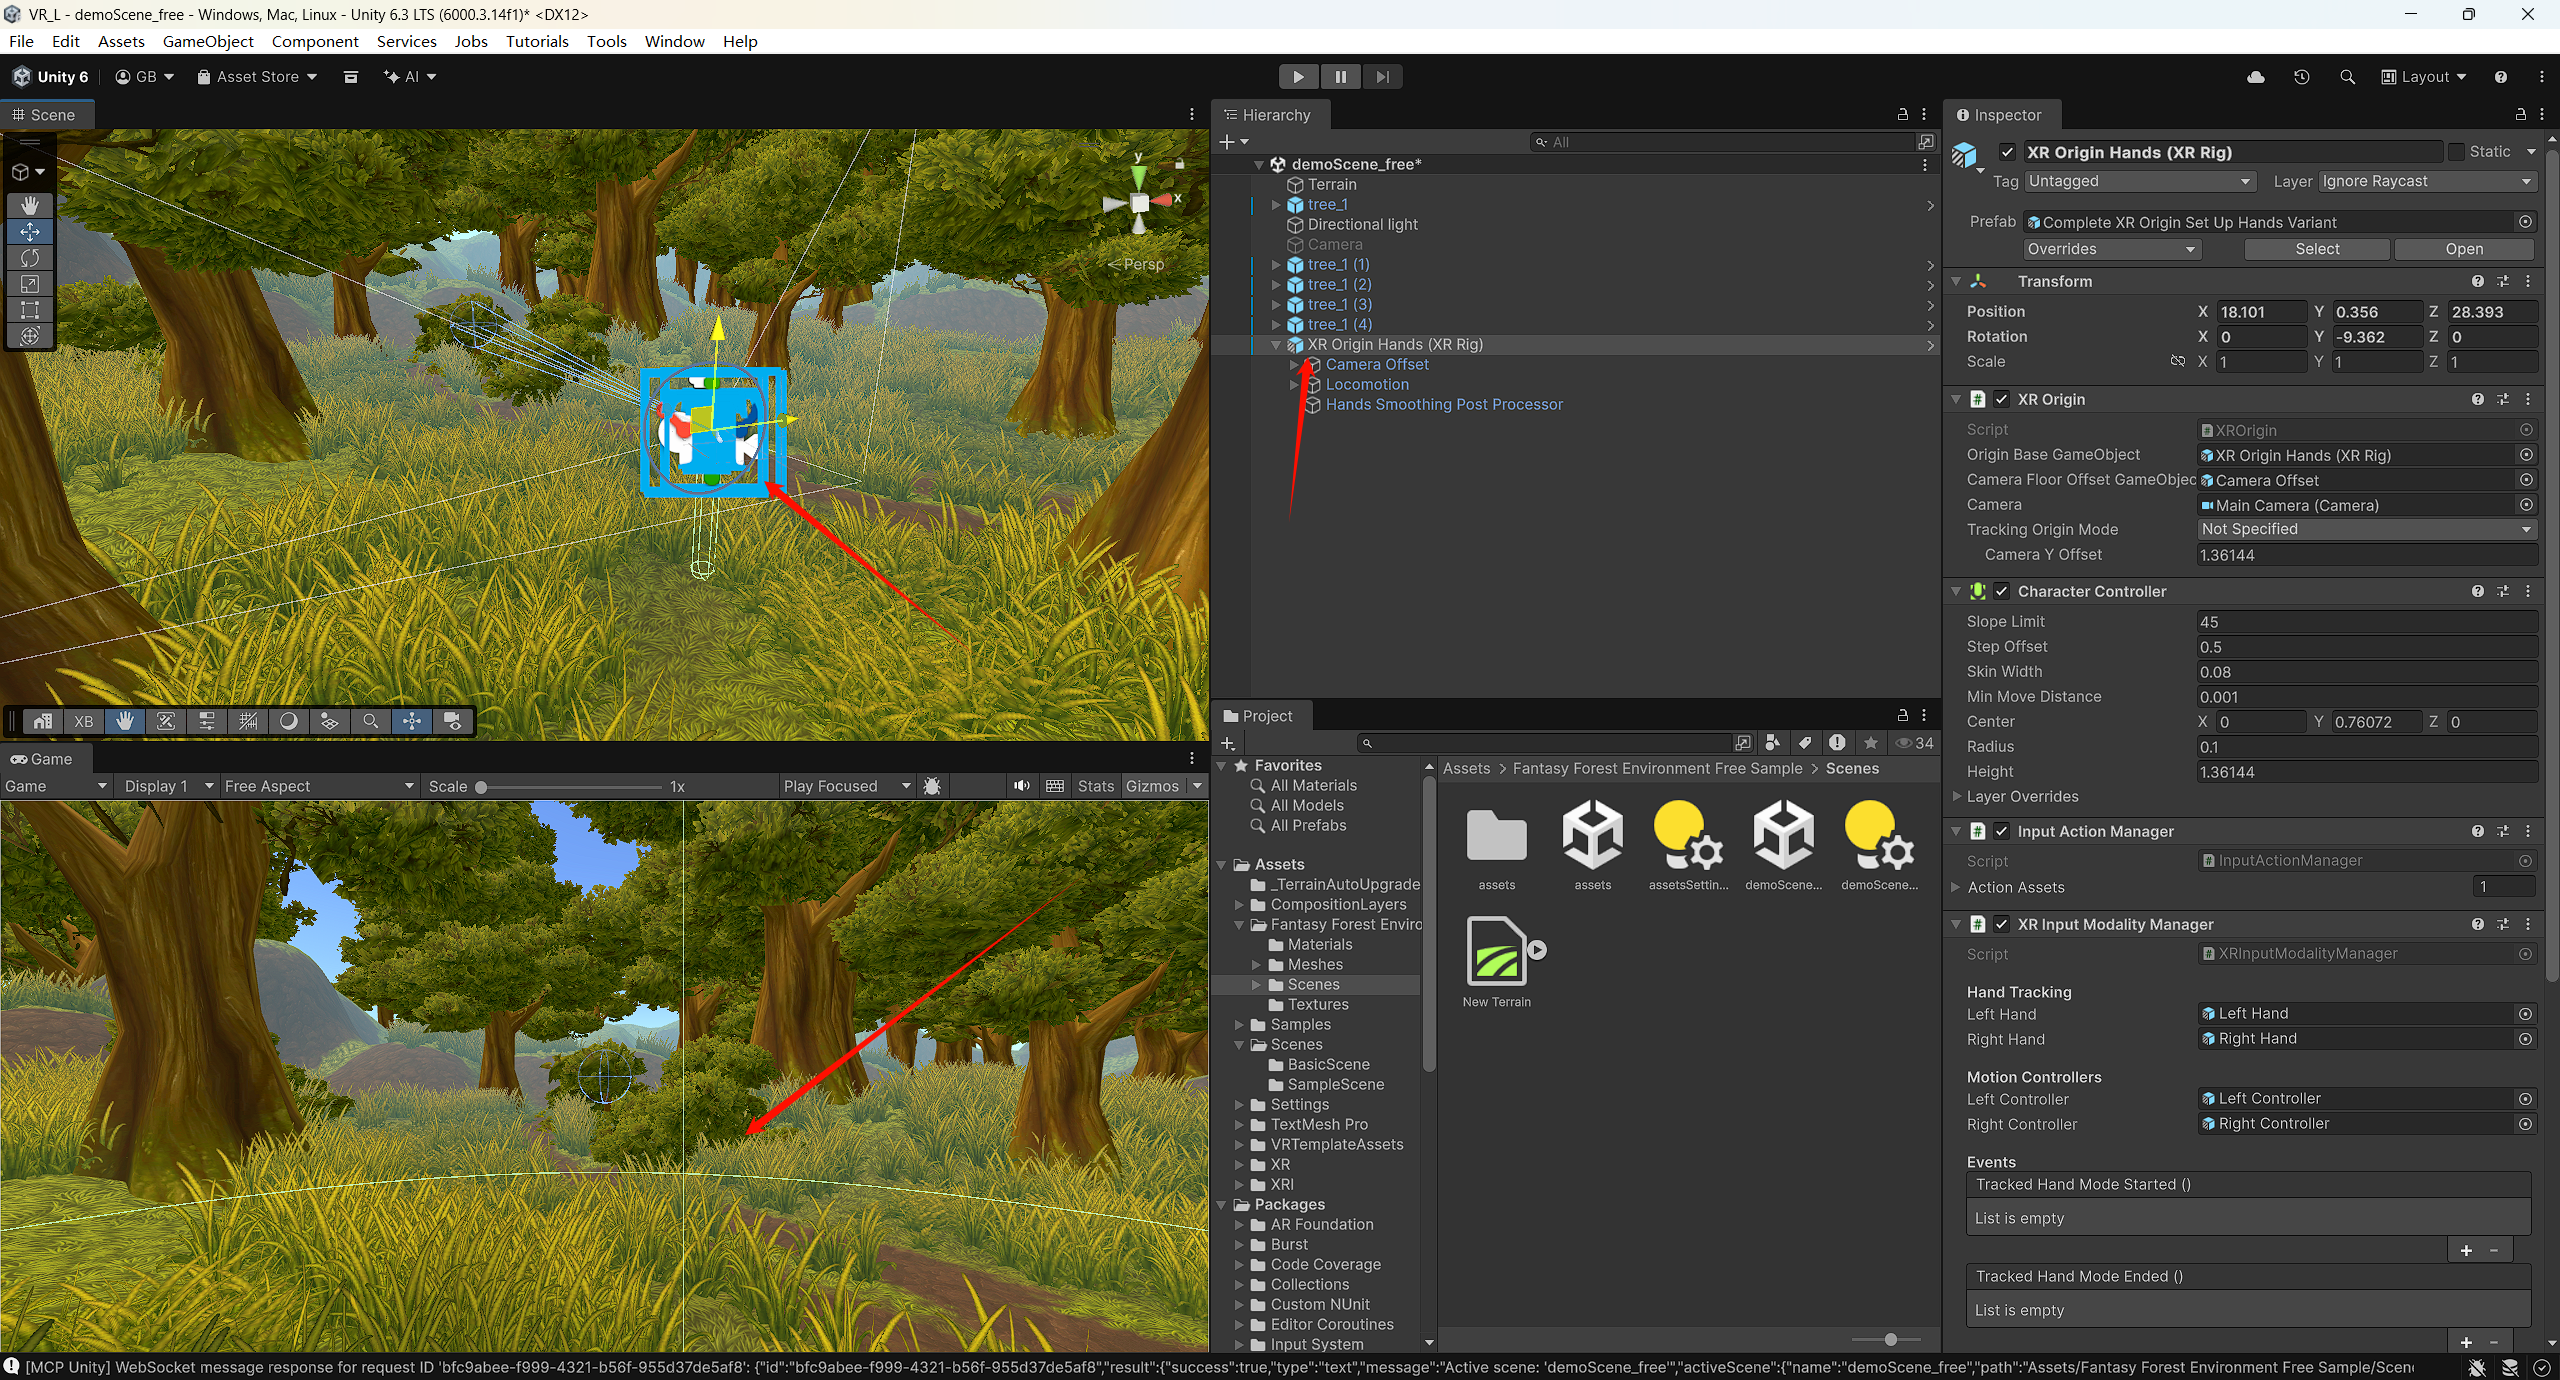
\includegraphics[width=0.86\textwidth]{img/chapter3/把vr视角复制进来.png}
  \caption{将 VR 模板中的 XR Origin 复制到森林场景}
  \label{fig:unity_copy_xr_origin}
\end{figure}

\subsubsection{调整出生点与相机冲突}

为了让进入场景后的观察位置合理，XR Origin 的位置参考森林场景原普通相机的位置设置：

\begin{itemize}
  \item X：\mintinline{text}|17.5541019|
  \item Y：\mintinline{text}|0|
  \item Z：\mintinline{text}|28.302784|
\end{itemize}

朝向参考原普通相机的水平朝向，将 Y 轴旋转设置为 \mintinline{text}|350.638153|。这样进入 VR 场景后，用户的初始视角能够面向森林环境主体，而不是偏离地形或植被区域。

同时，实验关闭了森林场景原来的普通 \mintinline{text}|Camera|。如果原相机和 XR Rig 内部的 \mintinline{text}|Main Camera| 同时存在并启用，可能出现多个主相机同时渲染、Audio Listener 冲突或 VR 视角被普通相机抢占的问题。关闭原相机后，场景由 XR Origin 内部的 \mintinline{text}|Main Camera| 负责显示，更符合 VR 模板的运行方式。

\subsection{运行展示与实验结果}

完成 Shader 修复、材质引用调整和 XR Origin 接入后，保存森林场景 \mintinline{text}|demoScene_free.unity|。验证结果表明，场景中已经存在 \mintinline{text}|XR Origin Hands (XR Rig)|，其内部包含 \mintinline{text}|Main Camera|、\mintinline{text}|Camera Offset|、手部、控制器、输入和移动相关组件；原普通 \mintinline{text}|Camera| 已设置为 inactive；Unity Console 当前没有错误。

从画面效果看，修复后的森林场景能够正常显示地形、树木、草地和植被材质，不再出现大面积粉色材质。由于场景中的地形已经带有 \mintinline{text}|TerrainCollider|，VR 玩家移动和重力检测可以依赖地形碰撞，具备进一步扩展交互功能的基础。

本章实验最终完成了一个基于 Unity VR 模板的森林场景展示流程。实验过程说明，VR 场景搭建不仅包括导入模型和摆放资源，还包括项目模板选择、渲染管线确认、资源包兼容性分析、Shader 修改、材质修复、XR Origin 接入和相机冲突处理。尤其是旧资源包迁移到新版本 URP 项目时，粉色材质问题不能只从外观上处理，而应追溯到 Shader 与渲染管线的兼容关系。

\subsection{本章小结}

本章以森林为主题，在 Unity 中完成了 VR 场景的创建与展示。实验先使用 VR 模板创建项目，再导入 Fantasy Forest Environment Free Sample 资源包。由于资源包主要面向旧 Built-in Render Pipeline，而当前项目使用 Unity 6 + URP 17.3.0，导入后出现大面积粉色材质。通过将资源包自带的 \mintinline{text}|StandardNoCulling.shader| 改写为 URP HLSL Shader，并调整相关材质引用，草地、树叶、树干和地面等资源恢复正常显示。

在场景交互方面，实验将 VR 模板中的完整 XR Origin 复制到森林样例场景，而不是只复制普通相机，从而保留 VR 相机、手部、控制器、输入和移动相关组件。最终，森林场景能够以 VR 视角进入和展示，为后续添加交互任务、路径漫游或识别结果可视化提供了基础。
